\subsection{Slučaj upotrebe: Praćenje napretka projekta}

\subsubsection*{Kratak opis}

Producent ili projektni menadžer prati koliko je film napredovao. Sistem prikazuje faze produkcije filma i koliko je koja faza završena, a za svaku fazu zadatke sa stanjem, članom tima i rokom. Zadaci kojima je prošao rok su posebno označeni i za njih se članu tima može poslati podsetnik.

\subsubsection*{Akteri}
\begin{itemize}
    \item \textbf{Producent}: prati napredak filma i šalje podsetnike članovima tima kada zadaci kasne.
    \item \textbf{Projektni menadžer}: prati napredak filma i šalje podsetnike članovima tima kada zadaci kasne.
\end{itemize}

\subsubsection*{Preduslovi}
\begin{itemize}
    \item Producent ili projektni menadžer je prijavljen na sistem.
    \item Film postoji u sistemu (slučaj upotrebe ,,Kreiranje filmskog projekta'').
    \item Za film su definisane faze produkcije (slučaj upotrebe ,,Definisanje faza produkcije'').
\end{itemize}

\subsubsection*{Postuslovi}
\begin{itemize}
    \item Podaci o filmu i zadacima se ne menjaju.
    \item Ako je poslat podsetnik, on je sačuvan, a član tima je obavešten.
\end{itemize}

\subsubsection*{Osnovni tok}
\begin{enumerate}
    \item Producent ili projektni menadžer (u daljem tekstu korisnik) bira film.
    \item Sistem prikazuje faze produkcije filma i procenat završenosti svake faze.
    \item Korisnik bira fazu.
    \item Sistem prikazuje zadatke te faze sa stanjem, rokom i članom tima, ako su dodeljeni.
    \item Korisnik bira zadatak.
    \item Sistem prikazuje detalje zadatka i materijale koji su za njega predati.
\end{enumerate}

Koraci 3 do 6 se ponavljaju dok korisnik želi da pregleda još faza.

\subsubsection*{Podtokovi: /}

\subsubsection*{Alternativni tokovi}

\paragraph*{A1: Film nema zadataka}
\begin{itemize}
    \item U koraku 2 osnovnog toka, ako film nema nijedan zadatak, sistem o tome obaveštava korisnika i slučaj upotrebe se završava.
\end{itemize}

\paragraph*{A2: Prošao rok zadatka}
\begin{itemize}
    \item U koraku 4 osnovnog toka, ako je nekom zadatku iz faze prošao rok, a nije završen, sistem ga označava.
    \item Ako je zadatak u stanju ,,Dodeljen'', ,,U Radu'' ili ,,Za Doradu'', korisnik može da pošalje podsetnik članu tima kome je zadatak dodeljen (slučaj upotrebe ,,Slanje podsetnika članu tima''). Sistem čuva podsetnik i obaveštava člana.
    \item Nastavlja se korak 5 osnovnog toka.
\end{itemize}

\subsubsection*{Specijalni zahtevi}
\begin{itemize}
    \item Korisnik vidi samo filmove na kojima je angažovan.
    \item Korisnik može da izabere samo fazu koja ima zadatke.
    \item Procenat završenosti faze se računa na osnovu zadataka u stanju ,,Završen''.
\end{itemize}

\subsubsection*{Dodatne informacije}
\begin{itemize}
    \item Faze produkcije se definišu u slučaju upotrebe ,,Definisanje faza produkcije''.
    \item Stanja zadatka: ,,Kreiran'', ,,Dodeljen'', ,,U Radu'', ,,Predat Na Pregled'', ,,Za Doradu'' i ,,Završen''. Dijagram stanja zadatka je dat uz slučaj upotrebe ,,Kreiranje i dodeljivanje zadataka''.
\end{itemize}

\begin{figure}[H]
	\centering
	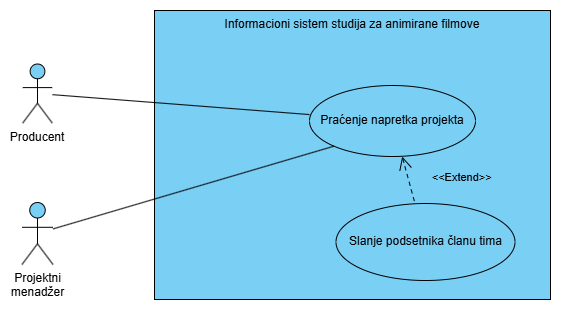
\includegraphics[width=\textwidth]{./dijagrami/dijagrami_slucajeva_upotrebe/pracenje_napretka_projekta.png}
	\caption{Dijagram slučaja upotrebe ,,Praćenje napretka projekta''}
 \end{figure}

\begin{figure}[H]
	\centering
	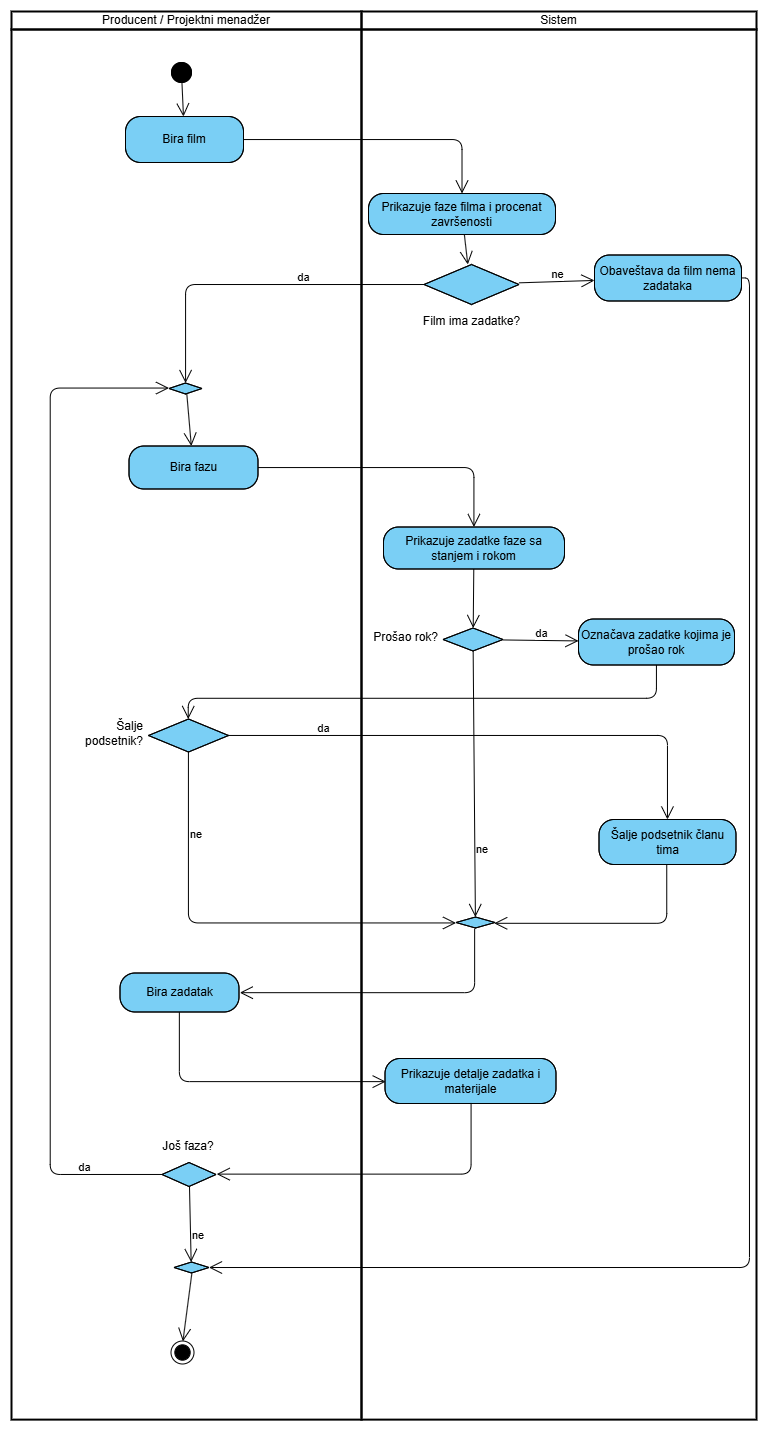
\includegraphics[width=\textwidth,height=0.85\textheight,keepaspectratio]{./dijagrami/dijagrami_aktivnosti/pracenje_napretka_projekta.png}
	\caption{Dijagram aktivnosti ,,Praćenje napretka projekta''}
 \end{figure}

\begin{figure}[H]
	\centering
	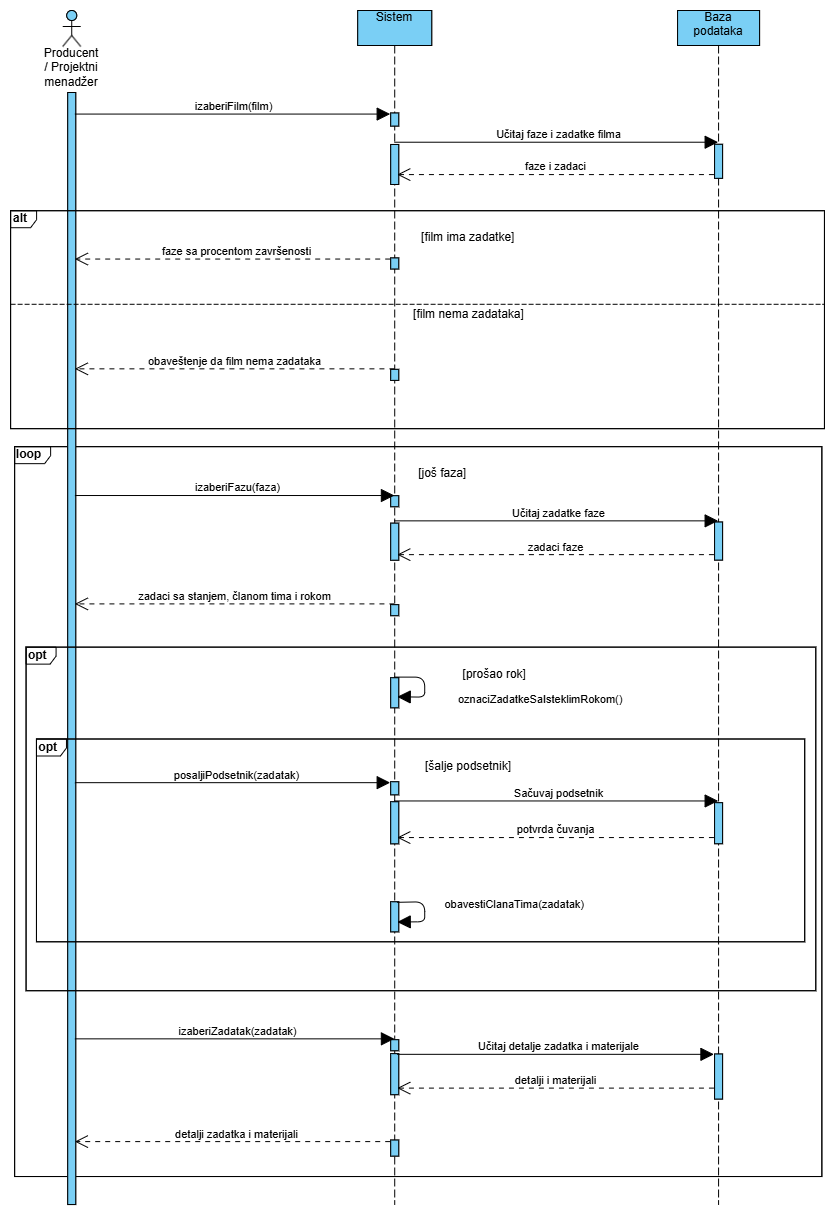
\includegraphics[width=\textwidth,height=0.9\textheight,keepaspectratio]{./dijagrami/dijagrami_sekvence/pracenje_napretka_projekta.png}
	\caption{Dijagram sekvence ,,Praćenje napretka projekta''}
 \end{figure}

\newpage
